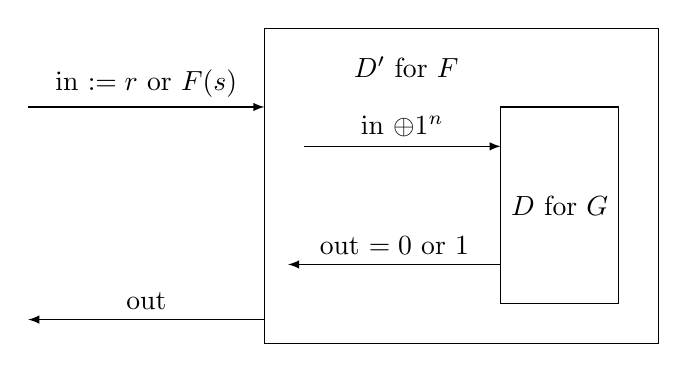
\begin{tikzpicture} %[scale=0.7, every node/.style={scale=0.7}]
\draw (0,0) rectangle (5,4);
\draw (3,0.5) rectangle (4.5,3);
\draw[-latex] (-3,3) -- (0,3) node [midway, above] {in $:= r$ or $F(s)$} node [midway, below] {};
\draw[-latex] (0,0.3) -- (-3,0.3) node [midway, above] {out};
\draw (1.8,3.5) node {$D'$ for $F$};
\draw (3.75,1.75) node {$D$ for $G$};
\draw[-latex] (0.5,2.5) -- (3,2.5) node [midway, above] {in $\oplus 1^{n}$ } node [midway, below] {};
\draw[-latex] (3,1) -- (0.3,1) node [midway, above] {out $= 0$ or $1$};
\end{tikzpicture}